\setcounter{page}{1}
\section*{Zielsetzung}
Im Versuch 61 sollen die Grundlagen der Lasertechnik kennengelernt werden. Hierzu werden zunächst die
wichtigsten theoretischen Grundlagen erarbeitet und anschließend die Eigenschaften eines Helium-Neon-Lasers
experimentell untersucht.
\section{Theorie}
Anhand der Quellen \ref{} und \ref{} wird im folgenden die theoretische Funktionsweise eines Lasers
erläutert. Zur Untersuchung der Wechselwirkung eines Strahlungsfeldes mit einem System aus Atomen bzw. Molekülen
wird das theoretische Modell eines Zweiniveausystems verwendet.
\subsection{Zweinniveausystem}
Als vereinfachtes Modell soll ein System mit den Zuständen $\ket{1}$ und $\ket{2}$ und zugehörigen Energieeigenwerten
$E\ua{1}$ und $E\ua{2}$ (mit $E\ua{2}> E\ua{1}$) betrachtet werden. Ein externes Strahlungsfeld sei durch die spektrale Energiedichte $\rho(\nu)$
charakterisiert. Durch die induzierte Absorption eine Photons der Energie $h \nu = E\ua{2} - E\ua{1}$ kann das
System in den Zustand $\ket{2}$ angeregt werden. Die Wahrscheinlichkeit $P\ua{1\rightarrow 2}$ für diesen Prozess ist proportional
zur spektrale Energiedichte $\rho(\nu)$
\begin{equation}
  P\ua{1\rightarrow 2} = B\ua{1\rightarrow 2}\cdot\rho(\nu).
\end{equation}
Der Proportionalitätsfaktor $B\ua{1\rightarrow 2}$ wird als Einsteinkoeffizient der induzierten Absorption bezeichnet. Analog kann
eine induzierte Emission stattfinden mit der Wahrscheinlichkeit
\begin{equation}
  P\ua{2\rightarrow 1} = B\ua{2\rightarrow 1}\cdot\rho(\nu).
\end{equation}
Mit dem Einsteinkoeffizienten der indzierten Emission $B\ua{2\rightarrow1}$.
Das induzierte Photon stimmt in Energie, Phase und Ausbreitungsrichtung mit dem anregenden Photon überein.
Unabhängig vom externen Strahlungsfeld
kann auch spontan ein Photon emittiert werden
\begin{equation}
  P\ua{s} = A\ua{2 \rightarrow 1}.
\end{equation}
Mit dem Einsteinkoeffizienten der spontanen Emission $A\ua{2 \rightarrow 1}$. Im thermischen Gleichgewicht folgen die Besetzungszahlen
$n\ua{i}$ der Niveaus einer Boltzmann-Statistik
\begin{equation}
  n\ua{i} = \frac{g\ua{i}n}{Z}\exp\left\{-\frac{E\ua{i}}{k\ua{B}T}\right\}.
\end{equation}
Hierbei ist $n$ die Gesamtzahl der Systeme, $g\ua{i}$ das statistische Gewicht des Zustands $\ket{i}$ und $Z$ die Zustandssumme. Im thermischen
Gleichgewicht dominiert somit die Besetzung des Grundzustandes.

Die Aufgabe eines Lasers besteht nun darin, eine dauerhafte Verstärkung des Strahlungsfeldes zu erzeugen.

\subsection{Funktionsprinzip eines Lasers}
Ein Laser besteht prinzipiell aus einem aktiven Lasermedium, einer Pumpquelle und einem Resonator. Die Pumpquelle sorgt dafür, dass
angeregte Zustände im Medium häufiger auftreten, als der Grundzustand. Diese Situation wird als Besetzungsinversion bezeichnet. Als direkte
Folge finden im Medium mehr induzierte Emissionen als spontane Emissionen statt, was dazu führt, dass das Strahlungsfeld durch das Medium verstärkt wird.
Der Resonator bewirkt, dass der Laufweg der Photonen im Medium verlängert wird. Das Prinzip ist in Abbildung \ref{fig: prinzip_laser} dargestellt.

Optische Resonatoren sind durch gegenüberliegende Spiegel realisiert, von denen mindestens einer halbdurchlässig ist.






Eine stabile Modenverteilung
stellt sich ein, wenn die folgende Stabilitätbedingung erfüllt ist
\begin{equation}
  0 \leq g_1 g_2 \leq 1.
  \label{eq: stabilität}
\end{equation}
Wobei $g\ua{i} = 1 - L/r\ua{i}$ mit dem Abstand der Spiegel $L$ und dem jeweiligen Krümmungsradius $r\ua{i}$. Das Produkt $g_1g_2$
als Funktion des Spiegelsabstandes $L$ ist in Abbildung \ref{fig: stabilitätsbedingung} dargestellt.
Für $r_1 = \SI{1000}{\milli\meter}$ ist die Bedingung \eqref{eq: stabilität} erfüllt für
\begin{equation}
  \SI{0}{\meter}\leq L \leq \SI{1}{\meter} \quad\lor\quad \SI{1.4}{\meter}\leq L \leq \SI{2.4}{\meter}.
\end{equation}
Bzw. für $r_1 = \SI{1400}{\milli\meter}$
\begin{equation}
  \SI{0}{\meter} \leq L \leq \SI{2.8}{\meter}.
\end{equation}
\begin{figure}
  \centering
  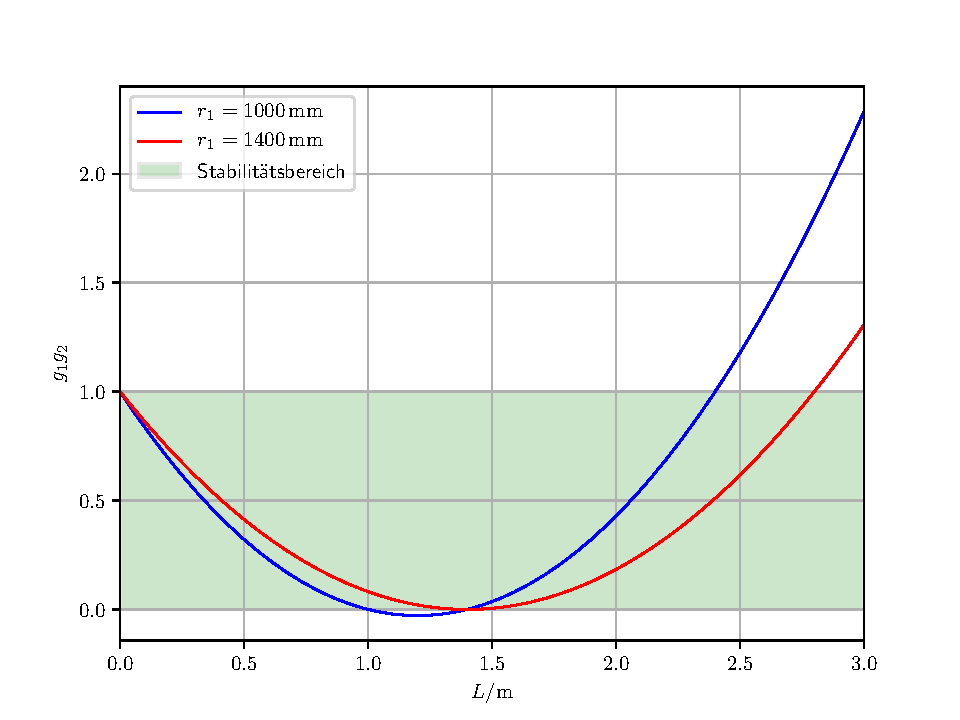
\includegraphics[width = \textwidth]{theorie_bilder/g_1_g_2.pdf}
  \caption{Darstsellung der Stabilitätsbedingung \eqref{eq: stabilität}. Hierbei gilt jeweils $r_2 = \SI{1400}{\milli\meter}$.}
  \label{fig: stabilitätsbedingung}
\end{figure}



\subsection{\ce{HeNe}-Laser }
